\documentclass[12pt,a4paper]{article}

\usepackage[a4paper,text={16.5cm,25.2cm},centering]{geometry}
\usepackage{lmodern}
\usepackage{amssymb,amsmath}
\usepackage{bm}
\usepackage{graphicx}
\usepackage{microtype}
\usepackage{hyperref}
\setlength{\parindent}{0pt}
\setlength{\parskip}{1.2ex}

\hypersetup
       {   pdfauthor = { Marco Fasondini },
           pdftitle={ foo },
           colorlinks=TRUE,
           linkcolor=black,
           citecolor=blue,
           urlcolor=blue
       }




\usepackage{upquote}
\usepackage{listings}
\usepackage{xcolor}
\lstset{
    basicstyle=\ttfamily\footnotesize,
    upquote=true,
    breaklines=true,
    breakindent=0pt,
    keepspaces=true,
    showspaces=false,
    columns=fullflexible,
    showtabs=false,
    showstringspaces=false,
    escapeinside={(*@}{@*)},
    extendedchars=true,
}
\newcommand{\HLJLt}[1]{#1}
\newcommand{\HLJLw}[1]{#1}
\newcommand{\HLJLe}[1]{#1}
\newcommand{\HLJLeB}[1]{#1}
\newcommand{\HLJLo}[1]{#1}
\newcommand{\HLJLk}[1]{\textcolor[RGB]{148,91,176}{\textbf{#1}}}
\newcommand{\HLJLkc}[1]{\textcolor[RGB]{59,151,46}{\textit{#1}}}
\newcommand{\HLJLkd}[1]{\textcolor[RGB]{214,102,97}{\textit{#1}}}
\newcommand{\HLJLkn}[1]{\textcolor[RGB]{148,91,176}{\textbf{#1}}}
\newcommand{\HLJLkp}[1]{\textcolor[RGB]{148,91,176}{\textbf{#1}}}
\newcommand{\HLJLkr}[1]{\textcolor[RGB]{148,91,176}{\textbf{#1}}}
\newcommand{\HLJLkt}[1]{\textcolor[RGB]{148,91,176}{\textbf{#1}}}
\newcommand{\HLJLn}[1]{#1}
\newcommand{\HLJLna}[1]{#1}
\newcommand{\HLJLnb}[1]{#1}
\newcommand{\HLJLnbp}[1]{#1}
\newcommand{\HLJLnc}[1]{#1}
\newcommand{\HLJLncB}[1]{#1}
\newcommand{\HLJLnd}[1]{\textcolor[RGB]{214,102,97}{#1}}
\newcommand{\HLJLne}[1]{#1}
\newcommand{\HLJLneB}[1]{#1}
\newcommand{\HLJLnf}[1]{\textcolor[RGB]{66,102,213}{#1}}
\newcommand{\HLJLnfm}[1]{\textcolor[RGB]{66,102,213}{#1}}
\newcommand{\HLJLnp}[1]{#1}
\newcommand{\HLJLnl}[1]{#1}
\newcommand{\HLJLnn}[1]{#1}
\newcommand{\HLJLno}[1]{#1}
\newcommand{\HLJLnt}[1]{#1}
\newcommand{\HLJLnv}[1]{#1}
\newcommand{\HLJLnvc}[1]{#1}
\newcommand{\HLJLnvg}[1]{#1}
\newcommand{\HLJLnvi}[1]{#1}
\newcommand{\HLJLnvm}[1]{#1}
\newcommand{\HLJLl}[1]{#1}
\newcommand{\HLJLld}[1]{\textcolor[RGB]{148,91,176}{\textit{#1}}}
\newcommand{\HLJLs}[1]{\textcolor[RGB]{201,61,57}{#1}}
\newcommand{\HLJLsa}[1]{\textcolor[RGB]{201,61,57}{#1}}
\newcommand{\HLJLsb}[1]{\textcolor[RGB]{201,61,57}{#1}}
\newcommand{\HLJLsc}[1]{\textcolor[RGB]{201,61,57}{#1}}
\newcommand{\HLJLsd}[1]{\textcolor[RGB]{201,61,57}{#1}}
\newcommand{\HLJLsdB}[1]{\textcolor[RGB]{201,61,57}{#1}}
\newcommand{\HLJLsdC}[1]{\textcolor[RGB]{201,61,57}{#1}}
\newcommand{\HLJLse}[1]{\textcolor[RGB]{59,151,46}{#1}}
\newcommand{\HLJLsh}[1]{\textcolor[RGB]{201,61,57}{#1}}
\newcommand{\HLJLsi}[1]{#1}
\newcommand{\HLJLso}[1]{\textcolor[RGB]{201,61,57}{#1}}
\newcommand{\HLJLsr}[1]{\textcolor[RGB]{201,61,57}{#1}}
\newcommand{\HLJLss}[1]{\textcolor[RGB]{201,61,57}{#1}}
\newcommand{\HLJLssB}[1]{\textcolor[RGB]{201,61,57}{#1}}
\newcommand{\HLJLnB}[1]{\textcolor[RGB]{59,151,46}{#1}}
\newcommand{\HLJLnbB}[1]{\textcolor[RGB]{59,151,46}{#1}}
\newcommand{\HLJLnfB}[1]{\textcolor[RGB]{59,151,46}{#1}}
\newcommand{\HLJLnh}[1]{\textcolor[RGB]{59,151,46}{#1}}
\newcommand{\HLJLni}[1]{\textcolor[RGB]{59,151,46}{#1}}
\newcommand{\HLJLnil}[1]{\textcolor[RGB]{59,151,46}{#1}}
\newcommand{\HLJLnoB}[1]{\textcolor[RGB]{59,151,46}{#1}}
\newcommand{\HLJLoB}[1]{\textcolor[RGB]{102,102,102}{\textbf{#1}}}
\newcommand{\HLJLow}[1]{\textcolor[RGB]{102,102,102}{\textbf{#1}}}
\newcommand{\HLJLp}[1]{#1}
\newcommand{\HLJLc}[1]{\textcolor[RGB]{153,153,119}{\textit{#1}}}
\newcommand{\HLJLch}[1]{\textcolor[RGB]{153,153,119}{\textit{#1}}}
\newcommand{\HLJLcm}[1]{\textcolor[RGB]{153,153,119}{\textit{#1}}}
\newcommand{\HLJLcp}[1]{\textcolor[RGB]{153,153,119}{\textit{#1}}}
\newcommand{\HLJLcpB}[1]{\textcolor[RGB]{153,153,119}{\textit{#1}}}
\newcommand{\HLJLcs}[1]{\textcolor[RGB]{153,153,119}{\textit{#1}}}
\newcommand{\HLJLcsB}[1]{\textcolor[RGB]{153,153,119}{\textit{#1}}}
\newcommand{\HLJLg}[1]{#1}
\newcommand{\HLJLgd}[1]{#1}
\newcommand{\HLJLge}[1]{#1}
\newcommand{\HLJLgeB}[1]{#1}
\newcommand{\HLJLgh}[1]{#1}
\newcommand{\HLJLgi}[1]{#1}
\newcommand{\HLJLgo}[1]{#1}
\newcommand{\HLJLgp}[1]{#1}
\newcommand{\HLJLgs}[1]{#1}
\newcommand{\HLJLgsB}[1]{#1}
\newcommand{\HLJLgt}[1]{#1}



\def\qqand{\qquad\hbox{and}\qquad}
\def\qqfor{\qquad\hbox{for}\qquad}
\def\qqas{\qquad\hbox{as}\qquad}
\def\half{ {1 \over 2} }
\def\D{ {\rm d} }
\def\I{ {\rm i} }
\def\E{ {\rm e} }
\def\C{ {\mathbb C} }
\def\R{ {\mathbb R} }
\def\H{ {\mathbb H} }
\def\Z{ {\mathbb Z} }
\def\CC{ {\cal C} }
\def\FF{ {\cal F} }
\def\HH{ {\cal H} }
\def\LL{ {\cal L} }
\def\vc#1{ {\mathbf #1} }
\def\bbC{ {\mathbb C} }



\def\fR{ f_{\rm R} }
\def\fL{ f_{\rm L} }

\def\qqqquad{\qquad\qquad}
\def\qqwhere{\qquad\hbox{where}\qquad}
\def\Res_#1{\underset{#1}{\rm Res}\,}
\def\sech{ {\rm sech}\, }
\def\acos{ {\rm acos}\, }
\def\asin{ {\rm asin}\, }
\def\atan{ {\rm atan}\, }
\def\Ei{ {\rm Ei}\, }
\def\upepsilon{\varepsilon}


\def\Xint#1{ \mathchoice
   {\XXint\displaystyle\textstyle{#1} }%
   {\XXint\textstyle\scriptstyle{#1} }%
   {\XXint\scriptstyle\scriptscriptstyle{#1} }%
   {\XXint\scriptscriptstyle\scriptscriptstyle{#1} }%
   \!\int}
\def\XXint#1#2#3{ {\setbox0=\hbox{$#1{#2#3}{\int}$}
     \vcenter{\hbox{$#2#3$}}\kern-.5\wd0} }
\def\ddashint{\Xint=}
\def\dashint{\Xint-}
% \def\dashint
\def\infdashint{\dashint_{-\infty}^\infty}




\def\addtab#1={#1\;&=}
\def\ccr{\\\addtab}
\def\ip<#1>{\left\langle{#1}\right\rangle}
\def\dx{\D x}
\def\dt{\D t}
\def\dz{\D z}
\def\ds{\D s}

\def\rR{ {\rm R} }
\def\rL{ {\rm L} }

\def\norm#1{\left\| #1 \right\|}

\def\pr(#1){\left({#1}\right)}
\def\br[#1]{\left[{#1}\right]}

\def\abs#1{\left|{#1}\right|}
\def\fpr(#1){\!\pr({#1})}

\def\sopmatrix#1{ \begin{pmatrix}#1\end{pmatrix} }

\def\endash{–}
\def\emdash{—}
\def\mdblksquare{\blacksquare}
\def\lgblksquare{\blacksquare}
\def\scre{\E}
\def\mapengine#1,#2.{\mapfunction{#1}\ifx\void#2\else\mapengine #2.\fi }

\def\map[#1]{\mapengine #1,\void.}

\def\mapenginesep_#1#2,#3.{\mapfunction{#2}\ifx\void#3\else#1\mapengine #3.\fi }

\def\mapsep_#1[#2]{\mapenginesep_{#1}#2,\void.}


\def\vcbr[#1]{\pr(#1)}


\def\bvect[#1,#2]{
{
\def\dots{\cdots}
\def\mapfunction##1{\ | \  ##1}
	\sopmatrix{
		 \,#1\map[#2]\,
	}
}
}



\def\vect[#1]{
{\def\dots{\ldots}
	\vcbr[{#1}]
} }

\def\vectt[#1]{
{\def\dots{\ldots}
	\vect[{#1}]^{\top}
} }

\def\Vectt[#1]{
{
\def\mapfunction##1{##1 \cr}
\def\dots{\vdots}
	\begin{pmatrix}
		\map[#1]
	\end{pmatrix}
} }

\def\addtab#1={#1\;&=}
\def\ccr{\\\addtab}

\def\questionequals{= \!\!\!\!\!\!{\scriptstyle ? \atop }\,\,\,}

\begin{document}

\textbf{Applied Complex Analysis (2021)}

\section{Lecture 7: Matrix norms and matrix functions}
This lecture we start to introduce an application of Cauchy's integral formula and trapezium rule: computing matrix functions, e.g., the matrix exponential $\E^A$. There are three possible definitions for matrix functions:

\begin{itemize}
\item[1. ] Taylor series


\item[2. ] Diagonalisation/Jordan canonical form


\item[3. ] Cauchy's integral formula

\end{itemize}
\subsection{Matrix norms}
Before discussing matrix functions we first review the notion of a matrix norm induced by a vector norm:

\[
\| A\| := \sup_{v : \| v \| = 1} \| A v\| = \sup_{v } {\| A v\| \over \| v\|}
\]
some examples of matrix norms are the 1-norm

\[
\|A \|_1 = \max_j \|A \vc e_j\|_1
\]
that is the maximum column sum, the $\infty$-norm

\[
\|A \|_\infty = \max_k \|A^\top \vc e_k\|_1
\]
that is the maximum row sum and the $2$-norm

\[
\|A \|_2
\]
which equals the largest singular value, or the square-root of the largest eigenvalue of $A^\top A$.

We denote the set of eigenvalues of a square matrix $A$, also known as the spectrum of $A$, by $\sigma(A)$. The \emph{spectral radius} of $A$ is defined as

\[
\rho(A) = \max\left\lbrace \vert \lambda \vert \: : \: \lambda \in \sigma(A)   \right\rbrace
\]
Hence,

\[
\|A \|_2 = \sqrt{\rho(A^\top A)}.
\]
Matrix norms have the usual norm properties, here  $\alpha$ is constant and $B$ has same dimensions as $A$:

\begin{itemize}
\item[1. ] \[
\|\alpha A\| = |\alpha| \| A \|
\]

\item[2. ] \[
\| A + B \| \leq \|A \| + \|B \|
\]
\end{itemize}
They have the extra feature that

\[
\|A B\| \leq \|A \| \|B \|
\]
which implies that

\[
\|A^k \| \leq \|A\|^k.
\]
\subsubsection{Taylor series definition}
One way to construct matrix exponentials is by Taylor series.

\textbf{Definition (Taylor series matrix function)} Suppose

\[
f(z) = \sum_{k=0}^\infty f_k z^k
\]
has radius of convergence $R$. If $\|A \| < R$ holds true for any matrix norm, then define

\[
f(A) := \sum_{k=0}^\infty f_k A^k.
\]
The well-posedness of this construction follows from the fact that the partial sums form a Cauchy sequence. In particular, let $\epsilon > 0$. Then for $r = \|A \| < R$ we can choose $N$ such that

\[
\sum_{k=n}^m |f_k| r^k \leq \epsilon
\]
for all $n,m > N$. Therefore

\[
\|\sum_{k=n}^m f_k A^k \| \leq \sum_{k=n}^m |f_k| \|A\|^k \leq \epsilon.
\]
The issue with Taylor series is that it requires analyticity to converge. We can see this clearly for the case $\sqrt{A}$ with Taylor series around $1$:

\[
\sqrt{z+1} = 1 + z/2 - z^2/8 + z^3/16 - \cdots = 1 + z/2 + \sum_{k=3}^\infty {3 \cdots (2k-3) \over 2^k k!} (-z)^k
\]
Consider


\begin{lstlisting}
(*@\HLJLk{using}@*) (*@\HLJLn{Plots}@*)(*@\HLJLp{,}@*) (*@\HLJLn{ComplexPhasePortrait}@*)(*@\HLJLp{,}@*) (*@\HLJLn{IntervalSets}@*)(*@\HLJLp{,}@*) (*@\HLJLn{LinearAlgebra}@*)
(*@\HLJLn{A}@*) (*@\HLJLoB{=}@*) (*@\HLJLp{[}@*)(*@\HLJLni{1}@*) (*@\HLJLnfB{0.1}@*)(*@\HLJLp{;}@*) (*@\HLJLnfB{0.2}@*) (*@\HLJLni{1}@*)(*@\HLJLp{]}@*)
(*@\HLJLn{\ensuremath{\lambda}}@*) (*@\HLJLoB{=}@*) (*@\HLJLnf{eigvals}@*)(*@\HLJLp{(}@*)(*@\HLJLn{A}@*)(*@\HLJLp{)}@*)
(*@\HLJLnf{phaseplot}@*)(*@\HLJLp{(}@*)(*@\HLJLoB{-}@*)(*@\HLJLnfB{2..2}@*)(*@\HLJLp{,}@*) (*@\HLJLoB{-}@*)(*@\HLJLnfB{1..1}@*)(*@\HLJLp{,}@*) (*@\HLJLn{z}@*) (*@\HLJLoB{->}@*) (*@\HLJLnf{sqrt}@*)(*@\HLJLp{(}@*)(*@\HLJLn{z}@*)(*@\HLJLp{))}@*)
(*@\HLJLnf{scatter!}@*)(*@\HLJLp{(}@*)(*@\HLJLnf{real}@*)(*@\HLJLp{(}@*)(*@\HLJLn{\ensuremath{\lambda}}@*)(*@\HLJLp{),}@*)(*@\HLJLnf{imag}@*)(*@\HLJLp{(}@*)(*@\HLJLn{\ensuremath{\lambda}}@*)(*@\HLJLp{);}@*) (*@\HLJLn{color}@*)(*@\HLJLoB{=:}@*)(*@\HLJLn{black}@*)(*@\HLJLp{)}@*)
\end{lstlisting}

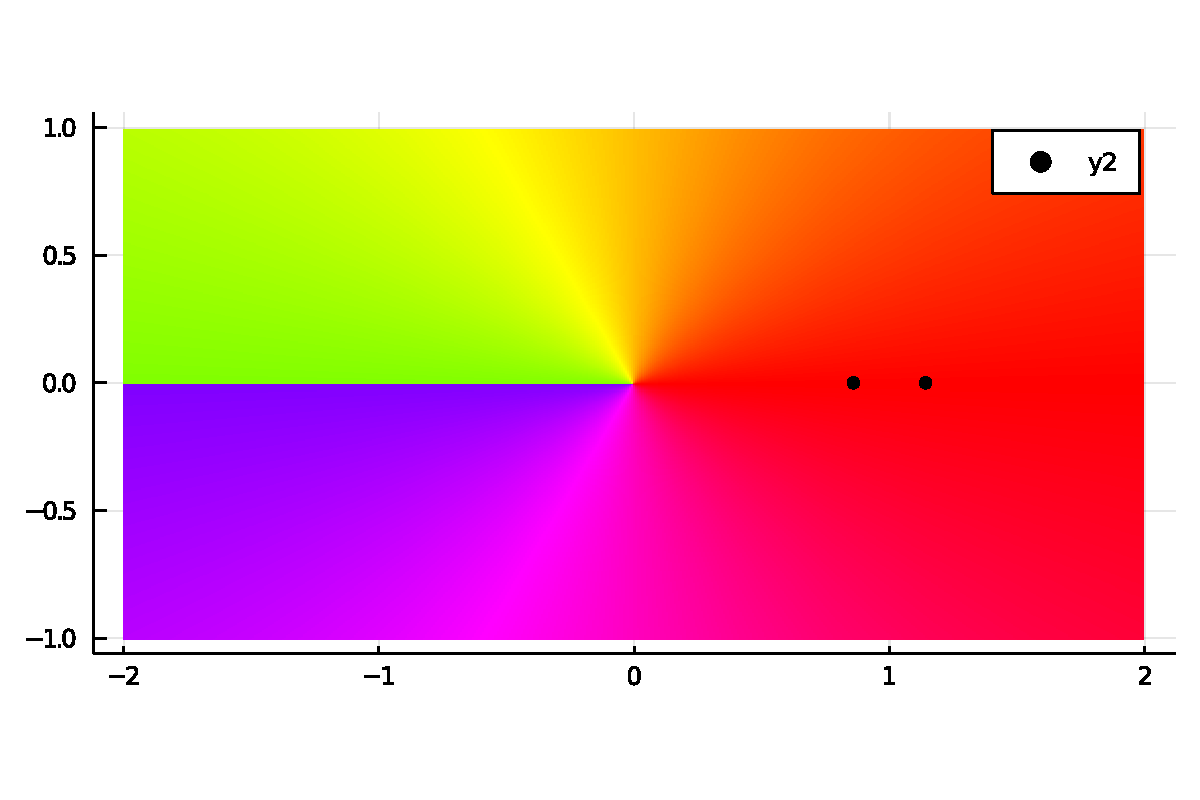
\includegraphics[width=\linewidth]{C:/Users/mfaso/OneDrive/Documents/GitHub/M3M6AppliedComplexAnalysis/output/figures/Lecture7_1_1.pdf}

Then, using a slightly modified \texttt{sqrt\_n} from Lecture 6 to compute the Taylor series and comparing with \texttt{sqrt(A)}, which is Julia's implementation of matrix square root, we see convergence, as the spectrum of \texttt{A} lies inside the disc of convergence of the Taylor series of $\sqrt{z}$ around 1:


\begin{lstlisting}
(*@\HLJLk{function}@*) (*@\HLJLnf{sqrt{\_}n}@*)(*@\HLJLp{(}@*)(*@\HLJLn{n}@*)(*@\HLJLp{,}@*)(*@\HLJLn{z}@*)(*@\HLJLp{,}@*)(*@\HLJLn{z\ensuremath{\_0}}@*)(*@\HLJLp{)}@*)
    (*@\HLJLn{ret}@*) (*@\HLJLoB{=}@*) (*@\HLJLnf{sqrt}@*)(*@\HLJLp{(}@*)(*@\HLJLn{z\ensuremath{\_0}}@*)(*@\HLJLp{)}@*) (*@\HLJLoB{*}@*) (*@\HLJLnf{one}@*)(*@\HLJLp{(}@*)(*@\HLJLn{z}@*)(*@\HLJLp{)}@*)
    (*@\HLJLn{c}@*) (*@\HLJLoB{=}@*) (*@\HLJLnfB{0.5}@*)(*@\HLJLoB{*}@*)(*@\HLJLnf{inv}@*)(*@\HLJLp{(}@*)(*@\HLJLn{ret}@*)(*@\HLJLp{)}@*)(*@\HLJLoB{*}@*)(*@\HLJLp{(}@*)(*@\HLJLn{z}@*)(*@\HLJLoB{-}@*)(*@\HLJLn{z\ensuremath{\_0}}@*)(*@\HLJLoB{*}@*)(*@\HLJLn{I}@*)(*@\HLJLp{)}@*)
    (*@\HLJLk{for}@*) (*@\HLJLn{k}@*)(*@\HLJLoB{=}@*)(*@\HLJLni{1}@*)(*@\HLJLoB{:}@*)(*@\HLJLn{n}@*)
        (*@\HLJLn{ret}@*) (*@\HLJLoB{+=}@*) (*@\HLJLn{c}@*)
        (*@\HLJLn{c}@*) (*@\HLJLoB{*=}@*) (*@\HLJLoB{-}@*)(*@\HLJLp{(}@*)(*@\HLJLni{2}@*)(*@\HLJLn{k}@*)(*@\HLJLoB{-}@*)(*@\HLJLni{1}@*)(*@\HLJLp{)}@*)(*@\HLJLoB{/}@*)(*@\HLJLp{(}@*)(*@\HLJLni{2}@*)(*@\HLJLoB{*}@*)(*@\HLJLp{(}@*)(*@\HLJLn{k}@*)(*@\HLJLoB{+}@*)(*@\HLJLni{1}@*)(*@\HLJLp{)}@*)(*@\HLJLoB{*}@*)(*@\HLJLn{z\ensuremath{\_0}}@*)(*@\HLJLp{)}@*)(*@\HLJLoB{*}@*)(*@\HLJLp{(}@*)(*@\HLJLn{z}@*)(*@\HLJLoB{-}@*)(*@\HLJLn{z\ensuremath{\_0}}@*)(*@\HLJLoB{*}@*)(*@\HLJLn{I}@*)(*@\HLJLp{)}@*)
    (*@\HLJLk{end}@*)
    (*@\HLJLn{ret}@*)
(*@\HLJLk{end}@*)
(*@\HLJLnf{norm}@*)(*@\HLJLp{(}@*)(*@\HLJLnf{sqrt}@*)(*@\HLJLp{(}@*)(*@\HLJLn{A}@*)(*@\HLJLp{)}@*) (*@\HLJLoB{-}@*) (*@\HLJLnf{sqrt{\_}n}@*)(*@\HLJLp{(}@*)(*@\HLJLni{100}@*)(*@\HLJLp{,}@*)(*@\HLJLn{A}@*)(*@\HLJLp{,}@*)(*@\HLJLni{1}@*)(*@\HLJLp{))}@*)
\end{lstlisting}

\begin{lstlisting}
7.738033469234878e-16
\end{lstlisting}


But  if the eigenvalues become much larger this won't work. Here we see an example of a matrix whose eigenvalues are not within the disc of convergence of the Taylor series:


\begin{lstlisting}
(*@\HLJLn{A}@*) (*@\HLJLoB{=}@*) (*@\HLJLp{[}@*)(*@\HLJLoB{-}@*)(*@\HLJLnfB{0.5}@*) (*@\HLJLoB{-}@*)(*@\HLJLni{4}@*)(*@\HLJLp{;}@*) (*@\HLJLni{3}@*) (*@\HLJLoB{-}@*)(*@\HLJLnfB{0.5}@*)(*@\HLJLp{]}@*)
(*@\HLJLn{\ensuremath{\lambda}}@*) (*@\HLJLoB{=}@*) (*@\HLJLnf{eigvals}@*)(*@\HLJLp{(}@*)(*@\HLJLn{A}@*)(*@\HLJLp{)}@*)
(*@\HLJLnf{phaseplot}@*)(*@\HLJLp{(}@*)(*@\HLJLoB{-}@*)(*@\HLJLnfB{2..2}@*)(*@\HLJLp{,}@*) (*@\HLJLoB{-}@*)(*@\HLJLnfB{5..5}@*)(*@\HLJLp{,}@*) (*@\HLJLn{z}@*) (*@\HLJLoB{->}@*) (*@\HLJLnf{sqrt}@*)(*@\HLJLp{(}@*)(*@\HLJLn{z}@*)(*@\HLJLp{))}@*)
(*@\HLJLnf{scatter!}@*)(*@\HLJLp{(}@*)(*@\HLJLnf{real}@*)(*@\HLJLp{(}@*)(*@\HLJLn{\ensuremath{\lambda}}@*)(*@\HLJLp{),}@*)(*@\HLJLnf{imag}@*)(*@\HLJLp{(}@*)(*@\HLJLn{\ensuremath{\lambda}}@*)(*@\HLJLp{);}@*) (*@\HLJLn{color}@*)(*@\HLJLoB{=:}@*)(*@\HLJLn{black}@*)(*@\HLJLp{,}@*) (*@\HLJLn{legend}@*)(*@\HLJLoB{=}@*)(*@\HLJLkc{false}@*)(*@\HLJLp{)}@*)
\end{lstlisting}

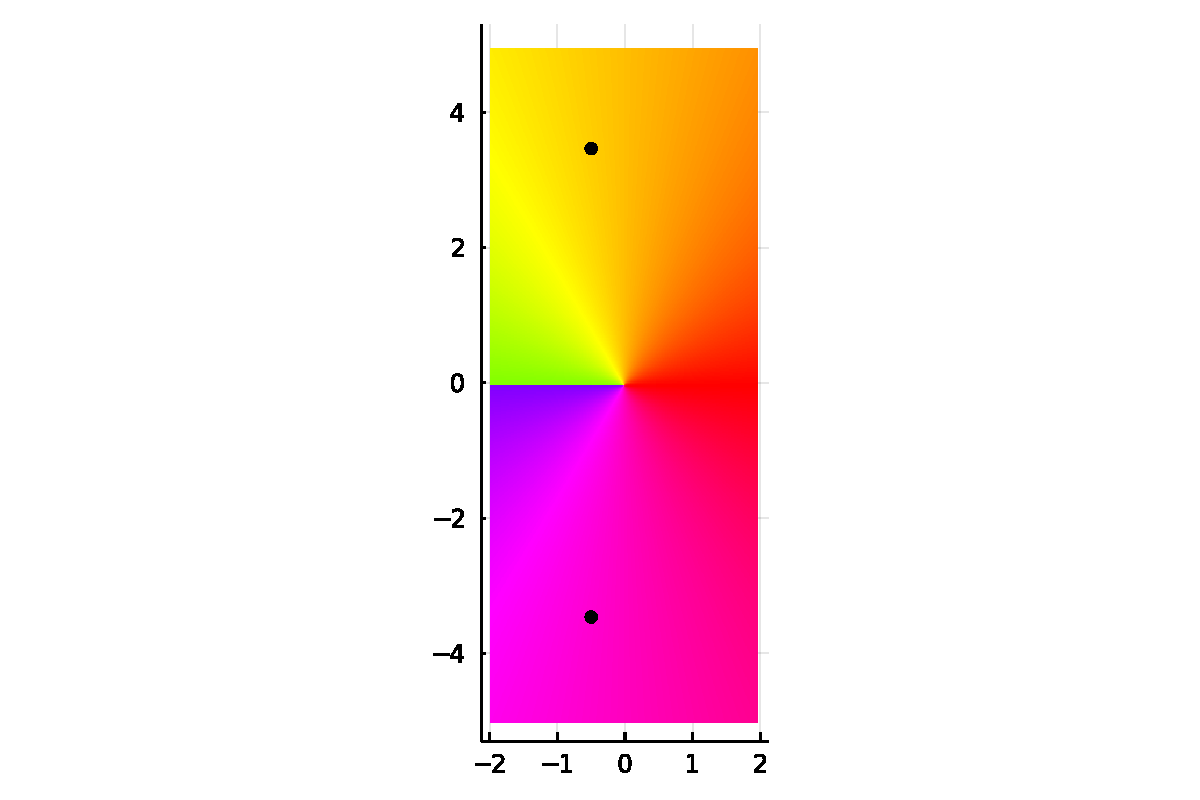
\includegraphics[width=\linewidth]{C:/Users/mfaso/OneDrive/Documents/GitHub/M3M6AppliedComplexAnalysis/output/figures/Lecture7_3_1.pdf}

Using the partial sum of the Taylor series completely fails, and catastrophically so:


\begin{lstlisting}
(*@\HLJLnf{norm}@*)(*@\HLJLp{(}@*)(*@\HLJLnf{sqrt}@*)(*@\HLJLp{(}@*)(*@\HLJLn{A}@*)(*@\HLJLp{)}@*) (*@\HLJLoB{-}@*) (*@\HLJLnf{sqrt{\_}n}@*)(*@\HLJLp{(}@*)(*@\HLJLni{100}@*)(*@\HLJLp{,}@*)(*@\HLJLn{A}@*)(*@\HLJLp{,}@*)(*@\HLJLni{1}@*)(*@\HLJLp{))}@*)
\end{lstlisting}

\begin{lstlisting}
2.1239250131186014e54
\end{lstlisting}


\subsection{Diagonalisation/Jordan canonical form}
\textbf{Definition (Diagonalisation of a matrix function)} Suppose $A = V \Lambda V^{-1}$ where

\[
\Lambda = \begin{pmatrix} \lambda_1 \\ & \ddots \\ && \lambda_d \end{pmatrix}
\]
Then define

\[
f(A) := V f(\Lambda) V^{-1} = V \begin{pmatrix} f(\lambda_1) \\ & \ddots \\ && f(\lambda_d) \end{pmatrix} V^{-1}
\]
This works very well as a definition but is slow for large matrices and does not take advantage of sparsity.

We can extend it to Jordan canonical form:

\textbf{Definition (Jordan canonical form)} Suppose

\[
A = V \begin{pmatrix} J_1 \\ & \ddots & \\&&& J_{\tilde d} \end{pmatrix} V^{-1}
\]
where $J_k$ are Jordan blocks, that is,

\[
J_k = \begin{pmatrix} \lambda_k & 1 \\ & \ddots & \ddots \\ && \lambda_k & 1 \\ &&& \lambda_k \end{pmatrix}
\]
Then define

\[
f(A) := V \begin{pmatrix} f(J_1) \\ & \ddots \\ && f(J_{\tilde d}) \end{pmatrix} V^{-1}
\]
using

\[
f\fpr(
\begin{pmatrix} \lambda & 1 \\ & \ddots & \ddots \\ && \lambda & 1 \\ &&& \lambda \end{pmatrix}) =
\begin{pmatrix} f(\lambda) & f'(\lambda) & \cdots & f^{(m-1)}(\lambda)/(m-1)! \\
        & \ddots & \ddots & \vdots \\
            & & f(\lambda) & f'(\lambda)\\
            &&& f(\lambda)
            \end{pmatrix}.
\]
This definition can be verified to be consistent with Taylor series when both are valid by direct inspection. For example, we have

\[
\sopmatrix{
\lambda & 1 \\
& \lambda
}^k = \sopmatrix{
\lambda^k & k \lambda^{k-1}\\
& \lambda^k
}.
\]
\subsection{Cauchy's integral formula}
The last approach we detail in the next lecture is to use the Cauchy integral formula:

\textbf{Definition (Cauchy's integral  matrix function)} Suppose $\gamma$ is a simple, closed contour that surrounds the spectrum of $A$ and $f$ is analytic in the interior. Then define

\[
f(A) := {1 \over 2 \pi \I} \oint_\gamma f(\zeta)(\zeta I - A)^{-1} \D \zeta
\]
Here the integrand is a matrix-valued function, hence consider the integral as defined entrywise.

Before we explain where this comes from, we can test on a simple example.


\begin{lstlisting}
(*@\HLJLn{A}@*) (*@\HLJLoB{=}@*) (*@\HLJLp{[}@*)(*@\HLJLoB{-}@*)(*@\HLJLnfB{0.5}@*) (*@\HLJLoB{-}@*)(*@\HLJLni{4}@*)(*@\HLJLp{;}@*) (*@\HLJLni{3}@*) (*@\HLJLoB{-}@*)(*@\HLJLnfB{0.5}@*)(*@\HLJLp{]}@*)
(*@\HLJLn{\ensuremath{\lambda}}@*)(*@\HLJLoB{=}@*) (*@\HLJLnf{eigvals}@*)(*@\HLJLp{(}@*)(*@\HLJLn{A}@*)(*@\HLJLp{)}@*)
(*@\HLJLn{\ensuremath{\theta}}@*) (*@\HLJLoB{=}@*) (*@\HLJLnf{range}@*)(*@\HLJLp{(}@*)(*@\HLJLni{0}@*)(*@\HLJLp{,}@*)(*@\HLJLni{2}@*)(*@\HLJLn{\ensuremath{\pi}}@*)(*@\HLJLp{,}@*)(*@\HLJLn{length}@*)(*@\HLJLoB{=}@*)(*@\HLJLni{1000}@*)(*@\HLJLp{)}@*)
(*@\HLJLn{\ensuremath{\gamma}}@*) (*@\HLJLoB{=}@*) (*@\HLJLn{\ensuremath{\theta}}@*) (*@\HLJLoB{->}@*) (*@\HLJLp{(}@*)(*@\HLJLn{z}@*) (*@\HLJLoB{=}@*) (*@\HLJLnf{exp}@*)(*@\HLJLp{(}@*)(*@\HLJLn{im}@*)(*@\HLJLoB{*}@*)(*@\HLJLn{\ensuremath{\theta}}@*)(*@\HLJLp{);}@*)  (*@\HLJLni{2}@*)(*@\HLJLn{z}@*) (*@\HLJLoB{+}@*) (*@\HLJLn{z}@*)(*@\HLJLoB{{\textasciicircum}}@*)(*@\HLJLni{2}@*) (*@\HLJLoB{-}@*) (*@\HLJLnfB{1.5}@*)(*@\HLJLoB{/}@*)(*@\HLJLn{z}@*)(*@\HLJLp{)}@*) (*@\HLJLcs{{\#}}@*) (*@\HLJLcs{a}@*) (*@\HLJLcs{curve}@*) (*@\HLJLcs{containing}@*) (*@\HLJLcs{\ensuremath{\lambda}}@*)
(*@\HLJLnf{phaseplot}@*)(*@\HLJLp{(}@*)(*@\HLJLoB{-}@*)(*@\HLJLnfB{2..2}@*)(*@\HLJLp{,}@*) (*@\HLJLoB{-}@*)(*@\HLJLnfB{5..5}@*)(*@\HLJLp{,}@*) (*@\HLJLn{z}@*) (*@\HLJLoB{->}@*) (*@\HLJLnf{sqrt}@*)(*@\HLJLp{(}@*)(*@\HLJLn{z}@*)(*@\HLJLp{))}@*)
(*@\HLJLnf{scatter!}@*)(*@\HLJLp{(}@*)(*@\HLJLnf{real}@*)(*@\HLJLp{(}@*)(*@\HLJLn{\ensuremath{\lambda}}@*)(*@\HLJLp{),}@*)(*@\HLJLnf{imag}@*)(*@\HLJLp{(}@*)(*@\HLJLn{\ensuremath{\lambda}}@*)(*@\HLJLp{);}@*) (*@\HLJLn{color}@*)(*@\HLJLoB{=:}@*)(*@\HLJLn{black}@*)(*@\HLJLp{,}@*) (*@\HLJLn{legend}@*)(*@\HLJLoB{=}@*)(*@\HLJLkc{false}@*)(*@\HLJLp{)}@*)
(*@\HLJLnf{plot!}@*)(*@\HLJLp{(}@*)(*@\HLJLnf{real}@*)(*@\HLJLp{(}@*)(*@\HLJLn{\ensuremath{\gamma}}@*)(*@\HLJLoB{.}@*)(*@\HLJLp{(}@*)(*@\HLJLn{\ensuremath{\theta}}@*)(*@\HLJLp{)),}@*) (*@\HLJLnf{imag}@*)(*@\HLJLp{(}@*)(*@\HLJLn{\ensuremath{\gamma}}@*)(*@\HLJLoB{.}@*)(*@\HLJLp{(}@*)(*@\HLJLn{\ensuremath{\theta}}@*)(*@\HLJLp{));}@*) (*@\HLJLn{color}@*)(*@\HLJLoB{=:}@*)(*@\HLJLn{blue}@*)(*@\HLJLp{,}@*) (*@\HLJLn{arrow}@*)(*@\HLJLoB{=}@*)(*@\HLJLkc{true}@*)(*@\HLJLp{)}@*)
\end{lstlisting}

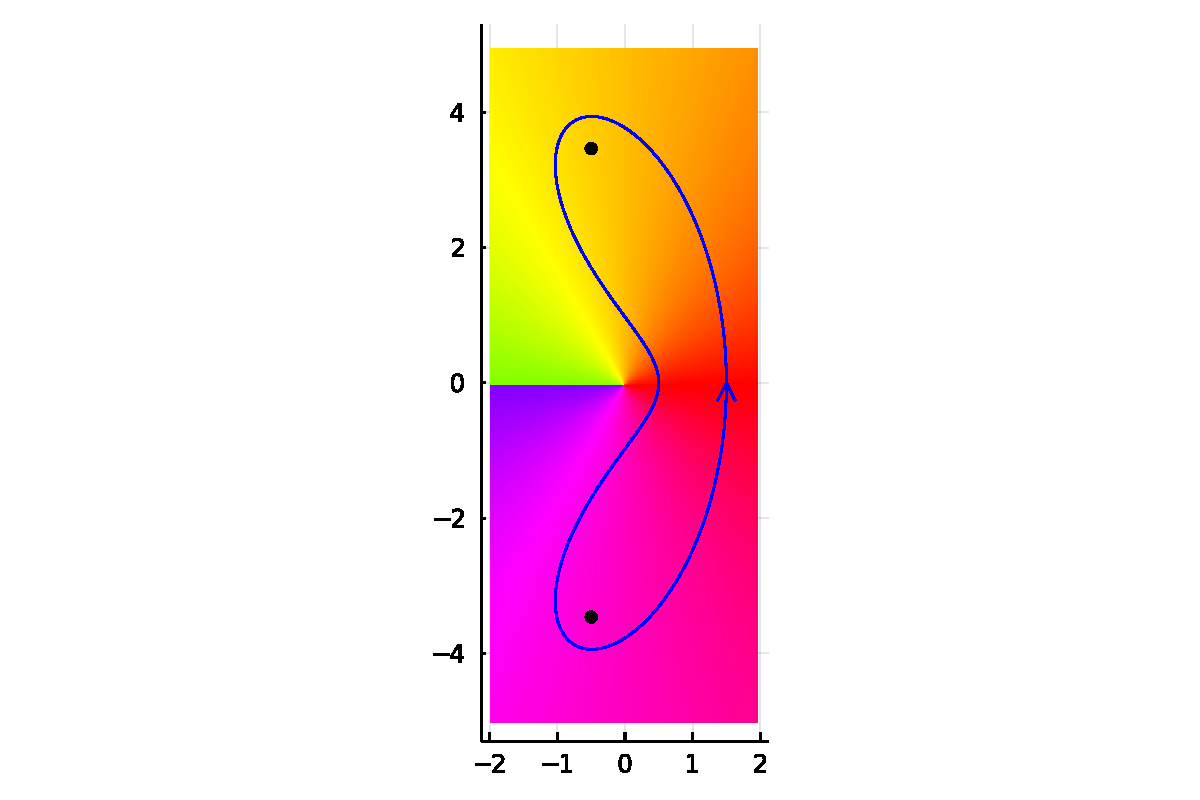
\includegraphics[width=\linewidth]{C:/Users/mfaso/OneDrive/Documents/GitHub/M3M6AppliedComplexAnalysis/output/figures/Lecture7_5_1.pdf}

We use the periodic Trapezium rule to integrate over the contour, showing it is valid:


\begin{lstlisting}
(*@\HLJLnf{periodic{\_}rule}@*)(*@\HLJLp{(}@*)(*@\HLJLn{N}@*)(*@\HLJLp{)}@*) (*@\HLJLoB{=}@*) (*@\HLJLni{2}@*)(*@\HLJLn{\ensuremath{\pi}}@*)(*@\HLJLoB{/}@*)(*@\HLJLn{N}@*)(*@\HLJLoB{*}@*)(*@\HLJLp{(}@*)(*@\HLJLni{0}@*)(*@\HLJLoB{:}@*)(*@\HLJLp{(}@*)(*@\HLJLn{N}@*)(*@\HLJLoB{-}@*)(*@\HLJLni{1}@*)(*@\HLJLp{)),}@*) (*@\HLJLni{2}@*)(*@\HLJLn{\ensuremath{\pi}}@*)(*@\HLJLoB{/}@*)(*@\HLJLn{N}@*)(*@\HLJLoB{*}@*)(*@\HLJLnf{ones}@*)(*@\HLJLp{(}@*)(*@\HLJLn{N}@*)(*@\HLJLp{)}@*)
(*@\HLJLn{\ensuremath{\gamma}p}@*) (*@\HLJLoB{=}@*) (*@\HLJLn{\ensuremath{\theta}}@*) (*@\HLJLoB{->}@*) (*@\HLJLp{(}@*)(*@\HLJLn{z}@*) (*@\HLJLoB{=}@*) (*@\HLJLnf{exp}@*)(*@\HLJLp{(}@*)(*@\HLJLn{im}@*)(*@\HLJLoB{*}@*)(*@\HLJLn{\ensuremath{\theta}}@*)(*@\HLJLp{);}@*) (*@\HLJLn{im}@*)(*@\HLJLoB{*}@*)(*@\HLJLn{z}@*)(*@\HLJLoB{*}@*)(*@\HLJLp{(}@*)(*@\HLJLni{2}@*) (*@\HLJLoB{+}@*) (*@\HLJLni{2}@*)(*@\HLJLn{z}@*) (*@\HLJLoB{+}@*) (*@\HLJLnfB{1.5}@*)(*@\HLJLoB{/}@*)(*@\HLJLn{z}@*)(*@\HLJLoB{{\textasciicircum}}@*)(*@\HLJLni{2}@*)(*@\HLJLp{))}@*)
(*@\HLJLn{N}@*) (*@\HLJLoB{=}@*) (*@\HLJLni{1000}@*)
(*@\HLJLn{\ensuremath{\theta}}@*)(*@\HLJLp{,}@*)(*@\HLJLn{w}@*) (*@\HLJLoB{=}@*) (*@\HLJLnf{periodic{\_}rule}@*)(*@\HLJLp{(}@*)(*@\HLJLn{N}@*)(*@\HLJLp{)}@*)

(*@\HLJLnf{norm}@*)(*@\HLJLp{(}@*)(*@\HLJLnf{sum}@*)(*@\HLJLp{(}@*)(*@\HLJLn{w}@*) (*@\HLJLoB{.*}@*) (*@\HLJLn{\ensuremath{\gamma}p}@*)(*@\HLJLoB{.}@*)(*@\HLJLp{(}@*)(*@\HLJLn{\ensuremath{\theta}}@*)(*@\HLJLp{)}@*)(*@\HLJLoB{.*}@*)(*@\HLJLn{sqrt}@*)(*@\HLJLoB{.}@*)(*@\HLJLp{(}@*)(*@\HLJLn{\ensuremath{\gamma}}@*)(*@\HLJLoB{.}@*)(*@\HLJLp{(}@*)(*@\HLJLn{\ensuremath{\theta}}@*)(*@\HLJLp{))}@*) (*@\HLJLoB{.*}@*) (*@\HLJLp{[}@*)(*@\HLJLnf{inv}@*)(*@\HLJLp{(}@*)(*@\HLJLnf{\ensuremath{\gamma}}@*)(*@\HLJLp{(}@*)(*@\HLJLn{\ensuremath{\theta}}@*)(*@\HLJLp{)}@*)(*@\HLJLoB{*}@*)(*@\HLJLn{I}@*)(*@\HLJLoB{-}@*)(*@\HLJLn{A}@*)(*@\HLJLp{)}@*) (*@\HLJLk{for}@*) (*@\HLJLn{\ensuremath{\theta}}@*) (*@\HLJLkp{in}@*) (*@\HLJLn{\ensuremath{\theta}}@*)(*@\HLJLp{])}@*)(*@\HLJLoB{/}@*)(*@\HLJLp{(}@*)(*@\HLJLni{2}@*)(*@\HLJLn{\ensuremath{\pi}}@*)(*@\HLJLoB{*}@*)(*@\HLJLn{im}@*)(*@\HLJLp{)}@*) (*@\HLJLoB{-}@*) (*@\HLJLnf{sqrt}@*)(*@\HLJLp{(}@*)(*@\HLJLn{A}@*)(*@\HLJLp{))}@*)
\end{lstlisting}

\begin{lstlisting}
1.6279683670392478e-15
\end{lstlisting}


We will discuss more next lecture.



\end{document}
